\documentclass [xcolor=svgnames, t] {beamer} 
\usepackage[utf8]{inputenc}
\usepackage{booktabs, comment} 
\usepackage[absolute, overlay]{textpos} 
\usepackage{pgfpages}
\usepackage[font=footnotesize]{caption}
\useoutertheme{infolines} 
\usepackage{advdate}
\definecolor{gold}{RGB}{254, 206, 0}

\setbeamercolor{title in head/foot}{bg=gray, fg=black}
\setbeamercolor{author in head/foot}{bg=myuniversity}
\setbeamertemplate{page number in head/foot}{}
\usepackage{csquotes}
\usepackage{multicol}
\usepackage{amsmath}
\usepackage[makeroom]{cancel}
\usepackage{bibentry}
\usepackage{multirow}
\usepackage{graphicx}
\usepackage{textpos}

\usepackage{tikz}

\usetheme{Madrid}
\definecolor{myuniversity}{RGB}{0, 85, 150}
\usecolortheme[named=myuniversity]{structure}
\usepackage{tikz}
\nobibliography*


\title[MTKD Presentation]{Multi-task Knowledge Distillation for Eye Disease Prediction}
\subtitle{Our implementation of Knowledge Distillation on Multi-task Learning}
\titlegraphic{
\includegraphics[height=2cm]{facultyLOGO.png}}
\author[Warsztaty Badawcze 2022L]{
	Mateusz Sperkowski, Szymon Rećko, Malwina Wojewoda}
\date{\today}

\addtobeamertemplate{navigation symbols}{}{%
    \usebeamerfont{footline}%
    \usebeamercolor[fg]{footline}%
    \hspace{1em}%
    \insertframenumber/\inserttotalframenumber
}

\begin{document}

{
\usebackgroundtemplate{
\includegraphics[height=\paperheight,width=\paperwidth]{black.png}}
\setbeamertemplate{navigation symbols}{}
\begin{frame}[plain]
\end{frame}
}

\begin{frame}
\maketitle
\end{frame}


\logo{
\includegraphics[scale=0.13]{logo.png}~%
}

\section{Introduction}
\begin{frame}{Paper Reproduction}
\centering
\textbf{\small “Non-reproducible single occurrences are of no significance to
science.”} 
{\footnotesize Karl Popper (1959), “The logic of scientific discovery”, p. 66}\\
\vspace{7mm}
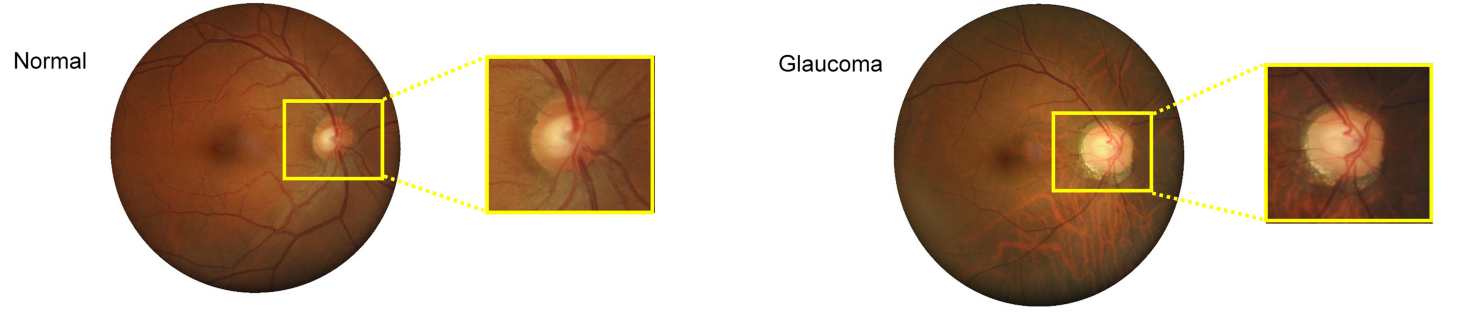
\includegraphics[width=\linewidth]{eye.png}
\vspace{5mm}
{\small \vspace{-2em} \bibentry{Chelaramani_2021_WACV}}
\end{frame}


\section{Table of Contents}
\begin{frame}
\frametitle{Table of Contents}
\tableofcontents
\end{frame}


\section{The Implementation}
\subsection{Used methods of Transfer Learning}
\begin{frame}{MTKD}
    \centering
\begin{figure}
\centering
\begin{minipage}{.5\textwidth}
  \centering
  \vspace{10mm}
  \begin{figure}[H]
  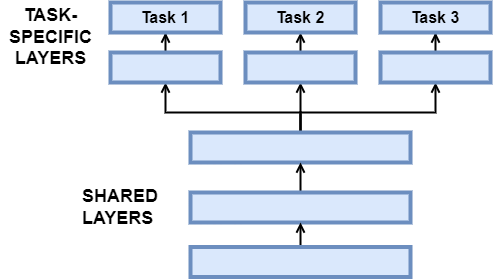
\includegraphics[width=.9\linewidth]{MTL scheme.png}
  \caption{Multi-task Learning}
  \end{figure}
\end{minipage}%
\begin{minipage}{.5\textwidth}
  \centering
  \vspace{10mm}
  \begin{figure}[H]
  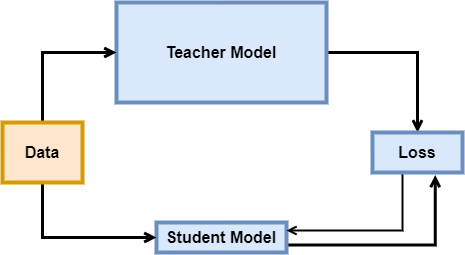
\includegraphics[width=\linewidth]{KD scheme.png}
  \caption{Knowledge distilation}
  \end{figure}
\end{minipage}
\end{figure}
\end{frame}

\begin{frame}{Pipeline Architecture}
\vspace{10mm}
    \centering
    \begin{figure}[H]
    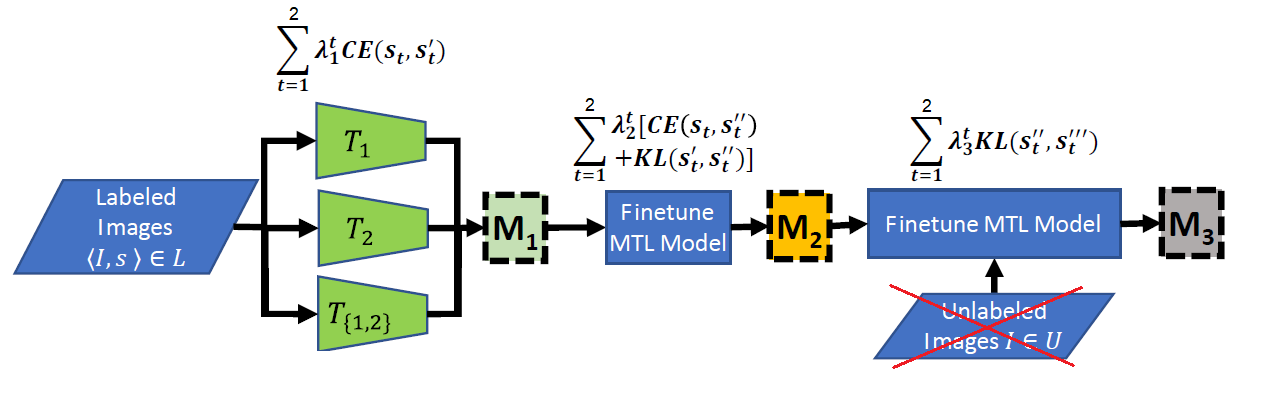
\includegraphics[width=1\textwidth]{pipe.png}
    \caption{Training phases of the MTKD Pipeline}
    \end{figure}
\end{frame}


\subsection{What worked and what didn't}
\begin{frame}{What worked and what didn't}
\begin{itemize}
    \item We managed to implement the Pipeline from the paper with reasonable changes. 
    \item We found labeled retinal fundus images similar to those used by the authors, with 2 similar tasks.

    \item We didn't manage to implement two other tasks.
    \item We didn't manage to thoroughly experiment on many hyperparameters and pretrained models.
    \item We had a problem with getting good results on model trained using KD.
    \item Crucial elements that were not described in the article:
    \begin{itemize}
        
        \item The shared layers from  pretrained ResNet-50.
        \item Weights in the sum of losses for Model 2.
        \item Precise method of ensembling the teachers.
        
    \end{itemize}
\end{itemize}

\end{frame}

\subsection{Our Results}
\begin{frame}{Results}
    \centering

\begin{table}[]
\begin{figure}[H]
\centering
\resizebox{\textwidth}{!}{%
\begin{tabular}{|c|cccc|cccc|}
\hline
\multirow{2}{*}{} &
  \multicolumn{4}{c|}{Task 1} &
  \multicolumn{4}{c|}{Task 2} \\ \cline{2-9} 
 &
  \multicolumn{2}{c|}{Balanced Accuracy} &
  \multicolumn{2}{c|}{F1} &
  \multicolumn{2}{c|}{Balanced Accuracy} &
  \multicolumn{2}{c|}{F1} \\ \hline
Model &
  \multicolumn{1}{l|}{Train} &
  \multicolumn{1}{l|}{Test} &
  \multicolumn{1}{l|}{Train} &
  \multicolumn{1}{l|}{Test} &
  \multicolumn{1}{l|}{Train} &
  \multicolumn{1}{l|}{Test} &
  \multicolumn{1}{l|}{Train} &
  \multicolumn{1}{l|}{Test} \\ \hline
M1{[}1{]} &
  \multicolumn{1}{c|}{0.911} &
  \multicolumn{1}{c|}{0.822} &
  \multicolumn{1}{c|}{0.864} &
  0.715 &
  \multicolumn{1}{c|}{-} &
  \multicolumn{1}{c|}{-} &
  \multicolumn{1}{c|}{-} &
  - \\ \hline
M1{[}2{]} &
  \multicolumn{1}{c|}{-} &
  \multicolumn{1}{c|}{-} &
  \multicolumn{1}{c|}{-} &
  - &
  \multicolumn{1}{c|}{0.889} &
  \multicolumn{1}{c|}{0.811} &
  \multicolumn{1}{c|}{0.888} &
  0.789 \\ \hline
M1{[}1,2{]} &
  \multicolumn{1}{c|}{0.843} &
  \multicolumn{1}{c|}{0.758} &
  \multicolumn{1}{c|}{0.799} &
  0.755 &
  \multicolumn{1}{c|}{0.874} &
  \multicolumn{1}{c|}{0.854} &
  \multicolumn{1}{c|}{0.832} &
  0.772 \\ \hline
Ensemble &
  \multicolumn{1}{c|}{0.946} &
  \multicolumn{1}{c|}{0.861} &
  \multicolumn{1}{c|}{0.920} &
  0.791 &
  \multicolumn{1}{c|}{0.870} &
  \multicolumn{1}{c|}{0.837} &
  \multicolumn{1}{c|}{0.828} &
  0.743 \\ \hline
M2 &
  \multicolumn{1}{c|}{0.857} &
  \multicolumn{1}{c|}{0.2} &
  \multicolumn{1}{c|}{0.803} &
  0.291 &
  \multicolumn{1}{c|}{0.883} &
  \multicolumn{1}{c|}{0.456} &
  \multicolumn{1}{c|}{0.821} &
  0.322 \\ \hline
M3 &
  \multicolumn{1}{c|}{0.2} &
  \multicolumn{1}{c|}{0.197} &
  \multicolumn{1}{c|}{0.042} &
  0.116 &
  \multicolumn{1}{c|}{0.385} &
  \multicolumn{1}{c|}{0.327} &
  \multicolumn{1}{c|}{0.324} &
  0.291 \\ \hline
\end{tabular}%
}
\end{table}
\caption{Results of the trained models}
\end{figure}
\end{frame}

\subsection{Diagrams}
\begin{frame}{MTKD}
    \centering
\begin{figure}
\centering
\begin{minipage}{.5\textwidth}
  \centering
  \vspace{10mm}
  \begin{figure}[H]
  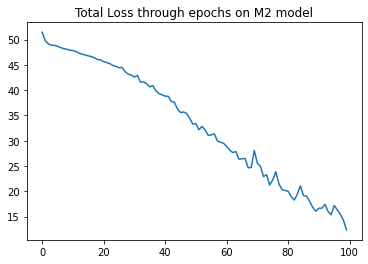
\includegraphics[width=0.9\linewidth]{M2_loss.png}
  \caption{Loss on M2}
  \end{figure}
\end{minipage}%
\begin{minipage}{.5\textwidth}
  \centering
  \vspace{10mm}
  \begin{figure}[H]
  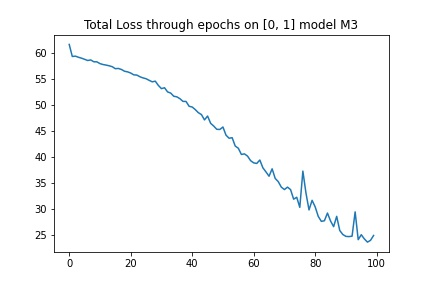
\includegraphics[width=1.1\linewidth]{M3_loss.jpg}
  \caption{Loss on M3}
  \end{figure}
\end{minipage}
\end{figure}
\end{frame}





\section{Pros$\And$Cons of the Architecture}
\begin{frame}{Pros$\And$Cons of the Architecture}
    \begin{multicols}{2}
    Pros :
    \begin{itemize}
    \vspace{14}
        \item  Possibility of using a small labelled dataset together with a larger unlabeled one.
        

        \\
        \item Potentially less costs connected to labeling a dataset.
        \\
        
        \item Teacher ensemble method is more effective than just a single teacher for KD.
    \end{itemize}
    \columnbreak
    Cons :
    \begin{itemize}
        \item High computing requirements for all task combinations. 
        \item Large number of hyperparameter choices.
        \item High requirements for in memory storage of the weights.
    \end{itemize}
    \end{multicols}
    
    \centering
\end{frame}

\section{Possible future expansions of project}
\begin{frame}{Possible future expansions of project}
\vspace{3mm}
Possible paths for improvements of the pipeline model.
\vspace{2mm}
   \begin{itemize}
        \item Expand model to the unused tasks.
       \item Generalize code for any dataset/model architectures.
       \item Test the architecture on other hyperparameters.
   \end{itemize}
\end{frame}

\begin{frame}{What we've learned}
\begin{itemize}
    \item Structure \& implementation of MTL and KD architectures
    \item Joining multiple loss functions
    \item Code and data sharing are crucial for reproduction
    \item Hyperparameters tuning
\end{itemize}
\end{frame}
    

\begin{frame}{Summary}
    \centering
    \begin{itemize}
    \item Reproduction is a crucial part of the scientific method and every scientist should strive to ensure that their paper is reproducible. In case of Computer Science, sharing the code is of upmost importance.
    \item We successfully analized and implemented a Multi-task Knowledge distillation pipeline.
    \item It's worth to consider joining multiple transfer learning methods for a single application.
    \end{itemize}
    \vspace{7mm}
    Feel free to send us questions (eg. MS Teams).\\ Thanks for listening!
\end{frame}
    

\begin{frame} [allowframebreaks]\frametitle{References}
\bibliographystyle{apalike}
\bibliography{bibfile}
\end{frame}

\end{document}